\documentclass[12pt, a4paper, oneside]{ctexart}
\usepackage{amsmath, amsthm, amssymb, bm, color, graphicx, geometry, hyperref, mathrsfs,extarrows, braket, booktabs, array}

\linespread{1.5}
%\geometry{left=2.54cm,right=2.54cm,top=3.18cm,bottom=3.18cm}
\geometry{left=1.84cm,right=1.84cm,top=2.18cm,bottom=2.18cm}
\newenvironment{problem}{\par\noindent\textbf{题目. }}{\bigskip\par}
\newenvironment{solution}{\par\noindent\textbf{解答. }}{\bigskip\par}
\newenvironment{note}{\par\noindent\textbf{注记. }}{\bigskip\par}

% 基本信息
\newcommand{\dt}{\today}
\newcommand{\sj}{实变函数}
\newcommand{\vt}{吴天阳 2204210460}

\begin{document}

%\pagestyle{empty}
\pagestyle{plain}
\vspace*{-15ex}
\centerline{\begin{tabular}{*3{c}}
    \parbox[t]{0.3\linewidth}{\begin{center}\textbf{日期}\\ \large \textcolor{blue}{\dt}\end{center}} 
    & \parbox[t]{0.3\linewidth}{\begin{center}\textbf{科目}\\ \large \textcolor{blue}{\sj}\end{center}}
    & \parbox[t]{0.3\linewidth}{\begin{center}\textbf{姓名,学号}\\ \large \textcolor{blue}{\vt}\end{center}} \\ \hline
\end{tabular}}
\vspace*{4ex}
\paragraph{5.1}求下列给定区间上关于权函数$\omega(x)$的正交多项式$g_0(x),g_1(x),g_2(x)$:

\begin{equation*}
    [0,1],\ \omega(x)=\sqrt{x}
\end{equation*}
\begin{solution}
    令$g_0(x) = 1$,则$\gamma_0 = (1, 1) = \int_0^1\sqrt{x}\,dx = \frac{2}{3}, \beta_0 = (x, 1)=\int_0^1x\sqrt{x}\,dx=\frac{2}{5}$,通过三项递推式可得
    \begin{equation*}
        g_1(x) = (x-\frac{\beta_0}{\gamma_0})g_0(x) = x-\frac{3}{5}
    \end{equation*}
    则
    \begin{equation*}
        \begin{aligned}
            \gamma_1 = &\ (x-\frac{3}{5},x-\frac{3}{5}) = \int_0^1\sqrt{x}(x-\frac{3}{5})(x-\frac{3}{5}) = \frac{2^3}{5^2\cdot 7}\\
            \beta_1 = &\ (x(x-\frac{3}{5}), x-\frac{3}{5}) = \int_0^1x\sqrt{x}(x-\frac{3}{5})(x-\frac{3}{5}) = \frac{2^3\cdot 23}{3^2\cdot 5^3\cdot 7}
        \end{aligned}
    \end{equation*}
    通过递推式可得
    \begin{equation*}
        \begin{aligned}
            g_2(x) = (x-\frac{\beta_1}{\gamma_1})g_1(x) - \frac{\gamma_1}{\gamma_0}g_0(x) =&\ \left(x-\frac{2^3\cdot 23}{3^2\cdot 5^3\cdot 7}\cdot\frac{5^2\cdot 7}{2^3}\right)(x-\frac{3}{5})-\frac{8}{5^2\cdot 7}\cdot \frac{3}{2} \\
            =&\ x^2-\frac{10}{9}x+\frac{5}{21}
        \end{aligned}
    \end{equation*}
    综上,
    \begin{equation*}
        \begin{aligned}
            g_0(x) = 1,\ g_1(x) = x-\frac{3}{5},\  g_2(x) = x^2-\frac{10}{9}x+\frac{5}{21}
        \end{aligned}
    \end{equation*}
\end{solution}

\paragraph{5.2}给定数据如下表中所示,求其最小二乘拟合函数$p(x)$:

(1) $p(x) = c_0+c_1x+c_2x^2$.
\renewcommand\arraystretch{0.6} % 设置表格高度为原来的0.8倍
\begin{table}[!htbp] % table标准
    \centering % 表格居中
    \begin{tabular}{p{1cm}<{\centering}p{1cm}<{\centering}p{1cm}<{\centering}p{1cm}<{\centering}p{1cm}<{\centering}p{1cm}<{\centering}p{1cm}<{\centering}p{1cm}<{\centering}p{1cm}<{\centering}p{1cm}<{\centering}} % 设置表格宽度
    %\begin{tabular}{cccc}
        \toprule
        $x_i$&1&3&4&5&6&7&8&9&10\\
        \midrule
        $y_i$&2&7&8&10&11&11&10&9&8\\
        \bottomrule
    \end{tabular}
\end{table}
\begin{solution}
    取$\phi_0(x) = 1, \phi_1(x) = x,\phi_2(x) = x^2$,则正规方程组为
    \begin{equation*}
        \left[\begin{matrix}
            9&53&381\\53&381&3017\\381&3017&25317
        \end{matrix}\right]
        \left[\begin{matrix}
            c_0\\c_1\\c_2
        \end{matrix}\right]=\left[\begin{matrix}
            76\\489\\3547
        \end{matrix}\right]
    \end{equation*}
    解得
    \begin{equation*}
        c_0 = -1.45966,\quad c_1 = 3.60531,\quad c_2 = -0.26757
    \end{equation*}
    所求的最小二乘拟合函数为
    \begin{equation*}
        p(x) = -1.45966+3.60531x-0.26757x^2
    \end{equation*}
\end{solution}
\paragraph{5.3}求下列函数在指定区间上的最优平方逼近一次多项式:

(1) $y=\sqrt{x},\ [0,1]$;\quad (2) $y=e^x,\ [-1,1]$.

\begin{solution}
    设$f=\sqrt{x}, p(x) = c_0+c_1x$,则$\phi_0(x) = 1,\phi_1(x) = x$,
    \begin{equation*}
        (\phi_i,\phi_j) = \int_0^1x^{i+j}\,dx = \frac{1}{i+j+1},\quad(\phi_i, f)=\int_0^1x^i\sqrt{x}=\frac{2}{2i+3}
    \end{equation*}
    由正规方程组有
    \begin{equation*}
        \left[\begin{matrix}
            1&1/2\\1/2&1/3
        \end{matrix}\right]\left[\begin{matrix}
            c_0\\c_1
        \end{matrix}\right]=\left[\begin{matrix}
            2/3\\2/5
        \end{matrix}\right]
    \end{equation*}
    解得
    \begin{equation*}
        c_0 = \frac{4}{15},\quad c_1 = \frac{4}{5}
    \end{equation*}
    所求的最优平方逼近一次多项式为
    \begin{equation*}
        p(x) = \frac{4}{15}+\frac{4}{5}x
    \end{equation*}

    (2) 设$f=e^{x}, p(x) = c_0+c_1x$,则$\phi_0(x) = 1,\phi_1(x) = x$,
    \begin{equation*}
        (\phi_i,\phi_j) = \int_{-1}^1x^{i+j}\,dx = \frac{1+(-1)^{i+j}}{i+j+1},\quad(\phi_0, f)=\int_{-1}^1e^x\,dx = e-\frac{1}{e},\quad (\phi_1,f)=\int_{-1}^1xe^x\,dx=\frac{2}{e}
    \end{equation*}
    由正规方程组有
    \begin{equation*}
        \left[\begin{matrix}
            2&0\\0&2/3
        \end{matrix}\right]\left[\begin{matrix}
            c_0\\c_1
        \end{matrix}\right]=\left[\begin{matrix}
            e-1/e\\2/e
        \end{matrix}\right]
    \end{equation*}
    解得
    \begin{equation*}
        c_0 = \frac{e}{2}-\frac{1}{2e},\quad c_1 = \frac{3}{e}
    \end{equation*}
    所求的最优平方逼近一次多项式为
    \begin{equation*}
        p(x) = \frac{e}{2}-\frac{1}{2e}+\frac{3}{e}x
    \end{equation*}
\end{solution}
\paragraph{5.4}利用正交多项式求下列函数的最优平方逼近二次多项式:
\begin{equation*}
    y = \arcsin x,\ [0,1].
\end{equation*}
\begin{solution}
    先计算几个积分的值为后面求值准备:
    \begin{equation*}
        \begin{aligned}
            I_0=&\ \int_0^1\arcsin x\,dx\xlongequal{x=\sin\theta}\int_0^{\pi/2}\theta\,d\sin\theta=\frac{\pi}{2}-1\\
            I_1=&\ \int_0^1x\arcsin x\,dx\xlongequal{x=\sin\theta}\frac{1}{2}\int_0^{\pi/2}\theta\sin2\theta\,d\theta=-\frac{1}{4}\int_0^{\pi/2}\theta\,d\cos 2\theta=\frac{\pi}{8}\\
            I_2=&\ \int_0^1x^2\arcsin x\,dx\xlongequal{x=\sin\theta}\int_0^{\pi/2}\theta\sin^2\theta\cos\theta\,d\theta=\int_0^{\pi/2}\frac{\theta}{2}(\cos\theta-\cos\theta\cos2\theta)\,d\theta\\
            =&\ \int_0^{\pi/2}\frac{\theta}{4}(\cos\theta-\cos3\theta)\,d\theta=\frac{1}{4}\left(\int_0^{\pi/2}\theta\,d\sin\theta-\frac{1}{3}\int_0^{\pi/2}\theta\,d\sin3\theta\right)=\frac{\pi}{6}-\frac{2}{9}
        \end{aligned}
    \end{equation*}
    通过三项递推的方式求解$[0,1]$上的二次正交多项式,令$g_0(x)=1,g_1(x)=x-\dfrac{\beta_0}{\gamma_0},g_2(x)=(x-\dfrac{\beta_1}{\gamma_1})g_1-\dfrac{\gamma_1}{\gamma_0}$,由于
    \begin{equation*}
        \beta_0=(x,1)=\int_0^1x\,dx=\frac{1}{2},\quad\gamma_0=(1,1)=\int_0^1\,dx=1
    \end{equation*}
    可知
    \begin{equation*}
        \begin{aligned}
            g_1(x)=x-\frac{1}{2},\quad &\ \beta_1=(x(x-\frac{1}{2}),x-\frac{1}{2})=\int_0^1x(x-\frac{1}{2})^2\,dx=\frac{1}{24},\\
            &\ \gamma_1=(x-\frac{1}{2},x-\frac{1}{2})=\int_0^1(x-\frac{1}{2})^2\,dx=\frac{1}{12}.
        \end{aligned}
    \end{equation*}
    则
    \begin{equation*}
        g_2(x) = (x-\frac{1}{24}\cdot 12)(x-\frac{1}{2})-\frac{1}{12} = x^2-x+\frac{1}{6},\quad \gamma_2=\int_0^1(x^2-x+\frac{1}{6})^2\,dx=\frac{1}{180}
    \end{equation*}

    设最优平方逼近二次多项式为$p(x)=c_0g_0(x)+c_1g_1(x)+c_2g_2(x)$,利用正交性,知$c_i=\dfrac{(f,g_i)}{(g_i,g_i)}$,从而得
    \begin{equation*}
        c_0 = \frac{I_0}{\gamma_0}=\frac{\pi}{2}-1,\quad c_1 = \frac{I_1}{\gamma_1}=\frac{3\pi}{2},\quad c_2=\frac{I_2}{\gamma_2}=30\pi-40
    \end{equation*}
    所求的最优平方逼近二次多项式为:
    \begin{equation*}
        \begin{aligned}
            p(x) =&\ \frac{\pi}{2}-1+\frac{3\pi}{2}(x-\frac{1}{2})+(30\pi-40)(x^2-x+\frac{1}{6})\\
            =&\ \frac{19\pi}{4}-\frac{23}{3}+(40-\frac{57\pi}{2})x+(30\pi-40)x^2
        \end{aligned}
    \end{equation*}
\end{solution}
\paragraph{5.5}取基函数为勒让德多项式,求函数$f(x)=\sin\frac{\pi}{2}x$在区间$[-1,1]$上的最优平方逼近三次多项式。
\begin{solution}
    通过三项递推式可求出$\text{Legendre}$多项式
    \begin{equation*}
        p_0(x) = 1,\quad p_1(x) = x,\quad p_2(x) = \frac{1}{2}(3x^2-1),\quad p_3(x) = \frac{1}{2}(5x^3-3x)
    \end{equation*}
    设最优平方逼近三次多项式为:$p(x) = c_0p_0(x)+c_1p_1(x)+c_2p_2(x)+c_3p_3(x)$,由$\text{Legendre}$多项式性质可知$(p_k,p_k)=\dfrac{2}{2k+1}$,则
    \begin{equation*}
        c_k=\frac{(f,p_k)}{(p_k,p_k)} = \frac{(f,p_k)\cdot(2k+1)}{2}
    \end{equation*}
    下面求解几个积分的值为后面计算准备:
    \begin{equation*}
        \begin{aligned}
            I_0 =&\ \int_{-1}^1\sin\frac{\pi}{2}x\,dx=0,\quad I_2 = \int_{-1}^1x^2\sin\frac{\pi}{2}x\,dx=0\\
            I_1 =&\ \int_{-1}^1x\sin\frac{\pi}{2}x\,dx=-\frac{2}{\pi}\int_{-1}^1x\,d\cos\frac{\pi}{2}x=\frac{8}{\pi^2}\\
            I_3 =&\ \int_{-1}^1x^3\sin\frac{\pi}{2}\,dx=-\frac{2}{\pi}\int_{-1}^1x^3\,d\cos\frac{\pi}{2}x=\frac{4}{\pi^2}\int_{-1}^13x^2\,d\sin\frac{\pi}{2}x = \frac{24}{\pi^2}(1-I_1)=\frac{24(\pi^2-8)}{\pi^4}
        \end{aligned}
    \end{equation*}
    则
    \begin{equation*}
        \begin{aligned}
            c_0=\frac{I_0}{2}=0,\quad c_1=\frac{3}{2}I_1=\frac{12}{\pi^2},\quad c_2=\frac{5(3I_2-I_0)}{4} = 0,\quad c_3=\frac{7(5I_3-3I_1)}{4}=\frac{168(\pi^2-10)}{\pi^4}
        \end{aligned}
    \end{equation*}
    所求的最优平方逼近三次多项式为:
    \begin{equation*}
        p(x) = \frac{12}{\pi^2}x+\frac{168(\pi^2-10)}{\pi^4}(\frac{1}{2}(5x^3-3x))=\frac{-240\pi^2+252}{\pi^4}x+\frac{420(\pi^2-10)}{\pi^4}x^3
    \end{equation*}
\end{solution}
\paragraph{5.6}求下列函数在指定区间上的最优一致逼近一次多项式:
\begin{equation*}
    y=\sqrt{x},\quad[\frac{1}{4},1]
\end{equation*}
\begin{solution}
    设$f(x) = y = \sqrt{x}$,则$f'(x) = \dfrac{1}{2\sqrt{x}},\ f''(x) = -\dfrac{1}{4}x^{-3/2}<0\ (x\in(1/4,1))$,令最优一致逼近一次多项式为:$p(x) = c_0+c_1x$,取偏差点$\tilde{x}_0 = 1/4, \tilde{x}_2=1$,则
    \begin{equation*}
        \begin{cases}
            \dfrac{1}{2} - c_0-\dfrac{1}{4}c_1=\mu\\
            \sqrt{\tilde{x}_1}-c_0-c_1\tilde{x}_1=-\mu\\
            1-c_0-c_1=\mu\\
            \dfrac{1}{2\sqrt{\tilde{x}_1}}-c_1=0
        \end{cases}
        \text{解得}
        \begin{cases}
            c_1=\dfrac{2}{3},\quad  \tilde{x}_1=\dfrac{1}{4c_1^2}=\dfrac{9}{16}\\
            c_0=\dfrac{1}{2}(\dfrac{1}{2}+\sqrt{\tilde{x}_1}-(\dfrac{1}{4}+\tilde{x}_1)c_1)=\dfrac{17}{48}\\
            \mu=1-c_0-c_1=-\dfrac{1}{48}
        \end{cases}
    \end{equation*}
    则$y=\sqrt{x}$在$[1/4,1]$上的最优一致逼近一次多项式为
    \begin{equation*}
        p(x) = \frac{17}{48}+\frac{2}{3}x\approx 0.35417+0.66667x
    \end{equation*}
    最大误差$E=-\mu = \dfrac{1}{48}\approx 0.02083$。
\end{solution}
\paragraph{5.10}用两种方法求下列函数在指定区间上的近似最优一致逼近一次式,并求其偏差:
\begin{equation*}
    y=e^{-x},\quad [-1,1].
\end{equation*}
\begin{solution}
    \textbf{法一}:$\text{Chebyshev}$插值多形式,$T_2(x)$的两个零点为
    \begin{equation*}
        x_0=\cos\dfrac{\pi}{4}=\dfrac{\sqrt{2}}{2},\ x_1=\cos\dfrac{3\pi}{4}=-\frac{\sqrt{2}}{2}
    \end{equation*}
    利用$\text{Newton}$插值多项式可知,近似最优一致逼近一次式为
    \begin{equation*}
        N_1(x) = y_0+\frac{y_1-y_0}{x_1-x_0}(x-x_0)=e^{-\frac{\sqrt{2}}{2}}+\frac{e^{\frac{\sqrt{2}}{2}}-e^{-\frac{\sqrt{2}}{2}}}{-\sqrt{2}}(x-\frac{\sqrt{2}}{2})\approx 1.2606-1.0854x
    \end{equation*}
    由$\text{Chebyshev}$插值多项式余项估计
    \begin{equation*}
        \max_{-1\leqslant x\leqslant 1}|R_1(x)|\leqslant\frac{M_2}{2!}\cdot\frac{1}{2}=\frac{e}{4} \approx 0.67957
    \end{equation*}
    其中$M_2=\max\limits_{-1\leqslant x\leqslant 1}|y''|=\max\limits_{-1\leqslant x\leqslant 1}e^{-x}=e$。
    
    \textbf{法二}:缩短幂级数法,将目标函数$\text{Tyalor}$展开至$2$次项
    \begin{equation*}
        e^{-x}=p_2(x)=1-x+\frac{1}{2}x^2+R_2(x)
    \end{equation*}
    且
    \begin{equation*}
        \max_{-1\leqslant x\leqslant 1}|R_2(x)| = \max_{-1\leqslant x\leqslant 1}\left|\frac{-e^{-x}}{3!}x^3\right|=\frac{e}{6}
    \end{equation*}
    由缩短幂级数法知,近似最优一致逼近一次式为
    \begin{equation*}
        p_1(x) = p_2(x) - \frac{1}{2}\cdot\frac{T_2(x)}{2} = 1-x+\frac{1}{2}x^2-\frac{1}{4}T_2=\frac{5}{4}-x=1.25-x
    \end{equation*}
    偏差估计为
    \begin{equation*}
        \max_{-1\leqslant x\leqslant 1}|R_2(x)|+\sup_{-1\leqslant x\leqslant 1}\frac{1}{4}T_2(x)\leqslant \frac{e}{6}+\frac{1}{4} \approx 0.70305
    \end{equation*}

\end{solution}

\paragraph{5.12}定义$T_k^*()=T_k(2x-1)$.

(1) 求$T_k^*(x)\ (k=0,1,2\cdot,4)$;

(2) 证明$T_k^*(x)$在区间$[0,1]$上关于权函数$\omega(x)=1/\sqrt{x-x^2}$正交;

(3) 证明$T_k^*(x^2)=T_{2k}(x)$。
\begin{solution}
    (1) \begin{equation*}
        \begin{aligned}
            &T_0^*(x) = T_0(2x-1)=1\\
            &T_1^*(x)=T_1(2x-1)=2x-1\\
            &T_2^*(x)=T_2(2x-1)=2(2x-1)^2-1=8x^2-8x+1\\
            &T_3^*(x) = 4(2x-1)^3-3(2x-1) = 32x^3-48x^2+18x-1\\
            &T_4^*(x) = 8(2x-1)^4-8(2x-1)^2+1=128x^4-256x^3+160x^2-32x+1
        \end{aligned}
    \end{equation*}
    
    (2) $\forall k, j\in\mathbb{N},\ k\neq j$,则
    \begin{equation*}
        \begin{aligned}
            \left(T_k^*(x),T_j^*(x)\right)=&\ \int_0^1\frac{\cos(k\, \arccos(2x-1))\cos(j\, \arccos(2x-1))}{\sqrt{x-x^2}}\,dx\\
            \xlongequal{2x-1=\cos t}&\ \int_0^\pi\frac{\cos(kt)\cos(jt)}{\sqrt{\frac{1+\cos t}{2}-\frac{(1+\cos t)^2}{4}}}\left(\frac{\sin t}{2}\right)\,dt\\
            =&\ \int_0^\pi\cos(kt)\cos(jt)\,dt=0
        \end{aligned}
    \end{equation*}

    (3) 设$x = \cos\theta, 2x^2-1=\cos\varphi$,则
    \begin{equation*}
        \begin{aligned}
            &\ \cos\varphi = 2\cos^2\theta-1=\cos 2\theta\\
            \Rightarrow&\ \varphi=\pm2\theta+2t\pi\quad(t\in\mathbb{Z})\\
            \Rightarrow&\ k\arccos(2x^2-1)=\pm2k\arccos x+2t\pi\quad (t\in\mathbb{Z})\\
            \Rightarrow&\ \cos(k\arccos(2x^2-1))=\cos(2k\arccos x)\\
            \Rightarrow&\ T_k^*(x^2)=T_{2k}(x)
        \end{aligned}
    \end{equation*}
\end{solution}

\iffalse
% 图片模板
\centerline{
    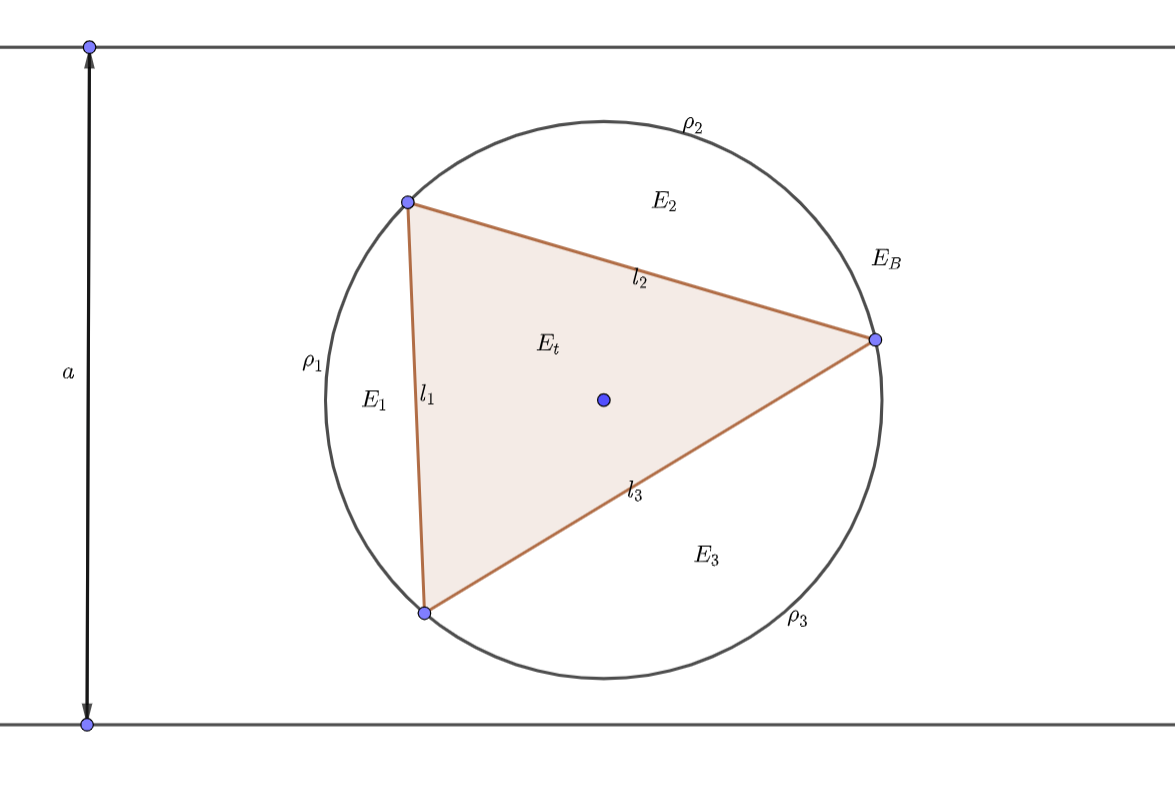
\includegraphics[width=0.8\textwidth]{figure.png}
}
\fi
\iffalse
% 表格模板
\renewcommand\arraystretch{0.8} % 设置表格高度为原来的0.8倍
\begin{table}[!htbp] % table标准
    \centering % 表格居中
    \begin{tabular}{p{1cm}<{\centering}p{1cm}<{\centering}p{3cm}<{\centering}p{5cm}<{\centering}} % 设置表格宽度
    %\begin{tabular}{cccc}
        \toprule
        $x_i$ & $f[x_1]$ & $f[x_i,x_{i+1}]$ & $f[x_i,x_{i+1},x_{i+2}]$ \\
        \midrule
        $x_0$ & $f(x_0)$ &                  &                          \\
        $x_0$ & $f(x_0)$ & $f'(x_0)$        &                          \\
        $x_0$ & $f(x_1)$ & $\frac{f(x_1)-f(x_0)}{x_1-x_0}$ & $\frac{f(x_1)-f(x_0)}{(x_1-x_0)^2}-\frac{f'(x_0)}{x_1-x_0}$\\
        \bottomrule
    \end{tabular}
\end{table}

\def\Log{\text{Log}} % 一个简单的宏定义
$\Log$ % 调用方法
\fi

\end{document}